% arara: clean: {
% arara: --> extensions:
% arara: --> ['aux', 'log', 'out', 'pdf']
% arara: --> }
% arara: lualatex: {
% arara: --> shell: yes,
% arara: --> draft: yes,
% arara: --> interaction: batchmode
% arara: --> }
% arara: lualatex: {
% arara: --> shell: yes,
% arara: --> draft: no,
% arara: --> interaction: batchmode
% arara: --> }
% arara: clean: {
% arara: --> extensions:
% arara: --> ['aux', 'log', 'out']
% arara: --> }
\documentclass[
	spanish,
	addpoints,
	answers,
	a4paper,
	11pt
]{exam}
\usepackage[spanish]{babel}
\usepackage[left=2cm,right=2cm,top=2cm,bottom=3cm]{geometry}
\usepackage{booktabs}
\usepackage{hhline}
\usepackage{array}
\usepackage{subfig}
\usepackage{duckuments}
\usepackage[intlimits]{mathtools}
\usepackage{amssymb}
\usepackage{diffcoeff}
\usepackage{amsthm}
\usepackage{pxfonts}
\usepackage[shortlabels]{enumitem}
\usepackage{multicol}
\usepackage{tikz}
\usepackage{hyperref}
\theoremstyle{definition}
\newtheorem{definition}{Definición}
\pagestyle{headandfoot}
\usepackage{emoji}
\usepackage[fixed]{fontawesome5}
\usepackage{minted}

\renewcommand{\solutiontitle}{\noindent\textcolor{AmurmapleBlue!80!black}{\sffamily\bfseries Solución}\par\noindent}
\renewcommand\listingscaption{Listado}
\newcommand{\unmarkedfntext}[1]{%
	\begingroup
	\renewcommand\thefootnote{}\footnote{#1}%
	\addtocounter{footnote}{-1}%
	\endgroup
}

% \difdef{c}{L}{op-symbol=\mathop{}\!\mathbin\bigtriangleup}
% \difdef{c}{A}{op-symbol=\mathop{}\!\mathbin\Box}

\pointpoints{Punto}{Puntos}
\bracketedpoints
\newcolumntype{C}{>{$}c<{$}}
\footer{}{Página \thepage\ de \numpages}{}


\def\logogem{%
	\begin{picture}(0,0)\unitlength=1cm
		\put(-11.5,-1){\href{https://fc.uni.edu.pe/estudios-de-grado/asociaciones-estudiantiles/gem}{
\includegraphics[width=2.8cm]{gem}}}
	\end{picture}
}

\def\logouni{%
	\begin{picture}(0,0)\unitlength=1cm
		\put(5,-1.2){
\includegraphics[width=2.4cm]{logouni}}
	\end{picture}
}

\unframedsolutions

\newcommand{\MVAt}{{\usefont{U}{mvs}{m}{n}\symbol{`@}}}
\definecolor{AmurmapleBlue}{RGB}{55,119,231}
\definecolor{AmurmapleOrange}{RGB}{230,108,17}
\definecolor{AmurmapleGreen}{rgb}{0.1,0.4,0.1}
\DeclareMathOperator{\sen}{sen}

\graphicspath{{../images/}}

\usetikzlibrary{babel}
\usetikzlibrary{arrows}
\usetikzlibrary{matrix}

\DeclareMathOperator{\Coker}{Koker}
\DeclareMathOperator{\Ker}{Ker}

\hypersetup{
	pdfencoding=auto,
	linktocpage=true,
	colorlinks=true,
	linkcolor=AmurmapleBlue!80!black,
	% citecolor=AmurmapleBlue!80!black,
	urlcolor=AmurmapleBlue!80!black,
	pdfpagelabels,
	pdftex,
	pdfauthor={Carlos Aznarán Laos},
	pdftitle={Taller de \LaTeX},
	pdfsubject={Taller de \LaTeX},
	pdfkeywords={pdf, programming},
	pdfproducer={LuaHBTeX, Version 1.22.0 (TeX Live 2026/dev/Arch Linux)},
	% bookmark=false
}


\begin{document}

\begin{center}
	\sffamily\bfseries
	\textcolor{AmurmapleBlue!80!black}{\Large Taller de \LaTeX}~\emoji{writing-hand-light-skin-tone}
	\logogem
	\logouni \\
	\textcolor{AmurmapleBlue!80!black}{Lista de Ejercicios de Reforzamiento}
\end{center}

\begin{center}
	\fbox{\fbox{\parbox{5.5in}
			{\centering
				Responda las preguntas en los espacios provistos en
				las hojas de preguntas.
				Los argumentos y la claridad de las respuestas se
				considerarán en la puntuación final.
			}}}
\end{center}
\vspace{0.1in}
\makebox[\textwidth]{Nombres y apellidos del alumno:\enspace\hrulefill}
\vspace{0.2in}
\makebox[\textwidth]{Nombres y apellidos del instructor:\enspace Carlos Aznarán.
	\textcolor{black}{\faIcon{inbox}}~\href{mailto:caznaranl@uni.pe}{\texttt{caznaranl\MVAt uni.pe}}\hfill}

\vspace*{-1.7\baselineskip}\setlength\belowdisplayshortskip{0pt}
\subsection*{\sffamily\color{AmurmapleBlue!80!black}Instrucciones}

\noindent
Descargue el material de la
\href{https://drive.google.com/drive/folders/1XrSPTzdgJXyY5q9rdA1zoEbKIxfG7LIR}{carpeta compartida\faGoogleDrive}.
Luego, suba los ficheros
\textcolor{AmurmapleBlue!80!black}{\mintinline{latex}|.tex|} con la
solución en el directorio \textcolor{AmurmapleBlue!80!black}{\sffamily Solución/Nombre Apellido}.

\begin{figure}[ht!]
	\centering
	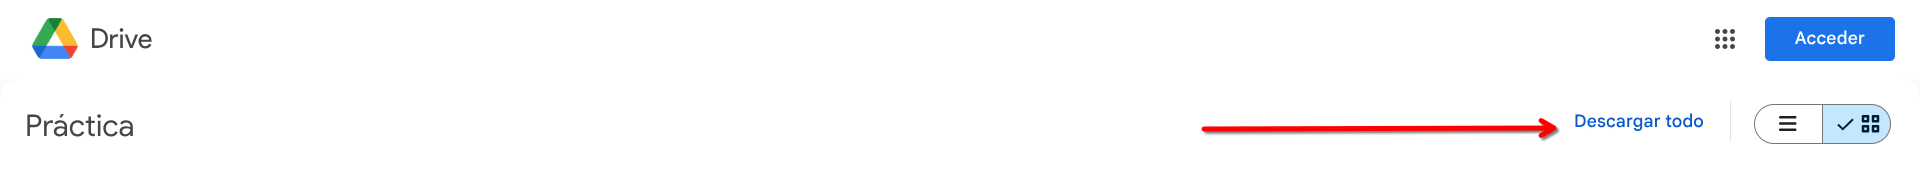
\includegraphics[width=.82\paperwidth]{drive}
\end{figure}

\vspace*{-1.7\baselineskip}\setlength\belowdisplayshortskip{0pt}
\subsection*{\sffamily\color{AmurmapleBlue!80!black}Ejercicios de clase~\emoji{teacher-light-skin-tone}}

\begin{questions}
	\question

Realice cada uno de los ejemplos de\href{https://drive.google.com/file/d/1OFmqAdh1-XTbVeuHS5Mn-c7aSAErCQe2/view}{\textcolor{red}{\faIcon{file-pdf}}\mintinline{latex}|t1.pdf|}:\href{https://drive.google.com/file/d/1rbNvSLlXMA1YnocPLROx05F6oJ-7Fvr6/view}{\textcolor{violet}{\faIcon{file}}\mintinline{latex}|helloworld.tex|},
\href{https://drive.google.com/file/d/1nL1XyMtPDasrUvjSZe6VIK8f1OXC1M9K/view}{\textcolor{violet}{\faIcon{file}}\mintinline{latex}|article.tex|},\href{https://drive.google.com/file/d/1s7p8jGuN_j0TmOr0vXCmb4ENJQFdZuhz/view}{\textcolor{violet}{\faIcon{file}}\mintinline{latex}|book.tex|},\\\href{https://drive.google.com/file/d/1FwOW64Jd24TQpoHid0SUy4QbpD6IntSU/view}{\textcolor{violet}{\faIcon{file}}\mintinline{latex}|report.tex|},\href{https://drive.google.com/file/d/1CcgX8S3e-8eVyT29JlFR4L6X_LVgXl9w/view}{\textcolor{violet}{\faIcon{file}}\mintinline{latex}|exam.tex|},\href{https://drive.google.com/file/d/1G0sE_5IZ3Di322UcV4XJAzcyRFH4tbyC/view}{\textcolor{violet}{\faIcon{file}}\mintinline{latex}|beamer.tex|} y\href{https://drive.google.com/file/d/1ACXGEDKyuMb4JJr4pZ_dlAeLPUnh9zbB/view}{\textcolor{violet}{\faIcon{file}}\mintinline{latex}|poster.tex|}.
En cada archivo, modifique\\\mintinline{latex}|\title{<Título>}| y \mintinline{latex}|\author{<Nombre>}|,
siempre que existan.

\question

Digite el ejercicio final de\href{https://drive.google.com/file/d/1OFmqAdh1-XTbVeuHS5Mn-c7aSAErCQe2/view}{\textcolor{red}{\faIcon{file-pdf}}\mintinline{latex}|t1.pdf|},
en el preámbulo incluya \mintinline{latex}|\documentclass{article}|.

\question

Importe \mintinline{latex}|\usepackage[shortlabels]{enumitem}|\footnote{Estudie la segunda sección de~\url{http://mirrors.ctan.org/macros/latex/contrib/enumitem/enumitem.pdf}}
y realice el ejemplo de listas numeradas de\href{https://drive.google.com/file/d/1O9foAwQ7XXrF28VHOq9FNcEt7kRHy3t5/view}{\textcolor{red}{\faIcon{file-pdf}}\mintinline{latex}|t2.pdf|}
con el entorno \mintinline{latex}|\begin{enumerate}[(i)]|.
¿Qué observa si crea las listas numeradas con el entorno
\mintinline{latex}|\begin{enumerate}[label=(\arabic*)]|?

\question

Importe \mintinline{latex}|\usepackage{siunitx}|\footnote{Estudie la tercera sección de~\url{http://mirrors.ctan.org/macros/latex/contrib/siunitx/siunitx.pdf}}
y cree una tabla de las magnitudes físicas fundamentales y otra tabla
de las magnitudes físicas derivadas, según el Sistema
Internacional\footnote{Vea~\url{https://en.wikipedia.org/wiki/International_System_of_Quantities}},
que indique en cada columna su nombre de la magnitud, su símbolo y su descripción.

\question

Importe \mintinline{latex}|\usepackage{xcolor}| y realice el espectro de
colores\footnote{Vea la tercera sección de \url{http://mirrors.ctan.org/macros/latex/contrib/xcolor/xcolor.pdf}}.

\begin{figure}[htbp]
	\centering
	\small
	\newcount\WL \unitlength.75pt
	\begin{picture}(460,60)(355,-10)
		\sffamily \tiny \linethickness{1.25\unitlength} \WL=360
		\multiput(360,0)(1,0){456}%
		{{\color[wave]{\the\WL}\line(0,1){50}}\global\advance\WL1}
		\linethickness{0.25\unitlength}\WL=360
		\multiput(360,0)(20,0){23}%
		{\picture(0,0)
			\line(0,-1){5} \multiput(5,0)(5,0){3}{\line(0,-1){2.5}}
			\put(0,-10){\makebox(0,0){\the\WL}}\global\advance\WL20
			\endpicture}
	\end{picture}
\end{figure}

\question

Digite el ejercicio final de\href{https://drive.google.com/file/d/1O9foAwQ7XXrF28VHOq9FNcEt7kRHy3t5/view}{\textcolor{red}{\faIcon{file-pdf}}\mintinline{latex}|t2.pdf|},
en el preámbulo incluya \mintinline{latex}|\documentclass{standalone}|.

\question

Digite la sección {\sffamily\color{AmurmapleBlue!80!black}1.6 The Gauss Transformation}
del\href{https://www.ceremade.dauphine.fr/~fejoz/Enseignement/ds2021/Brin-Stuck_2002_Introduction-to-Dynamical-Systems.pdf}{\textcolor{red}{\faIcon{file-pdf}}texto},
sin incluir los ejercicios.

\question

Importe \mintinline{latex}|\usepackage{diffcoeff}| y digite la
sección {\sffamily\color{AmurmapleBlue!80!black}Transformación de Hopf-Cole}
del\href{https://weblibrary.mila.edu.my/upload/ebook/engineering/2014_Book_IntroductionToPartialDifferent.pdf#page=338}{\textcolor{red}{\faIcon{file-pdf}}texto}
para transformar la ecuación potencial de Burgers en la ecuación de
difusión lineal.
\begin{equation*}
	\boxed{
		\diffp{v}{t}=
		\gamma\diffp[2]{v}{x}\quad
		\xRightarrow{v\left(t,x\right)=\exp\left(\alpha\varphi\left(t,x\right)\right)}\quad
		\diffp{\varphi}{t}=
		\gamma\diffp[2]{\varphi}{x}+
		\gamma\alpha{\left(\diffp{\varphi}{x}\right)}^{2}.
	}
\end{equation*}

\question

Importe \mintinline{latex}|\usepackage{subfig}| y realice el
siguiente mosaico de figuras (referenciales).

\begin{figure*}
	\captionsetup[figure]{margin=10pt}
	\subfloat[Primero izquierda.]{\includegraphics[width=.2\paperwidth]{example-image-duck}}
	\hfill
	\subfloat[Primero derecha.]{\includegraphics[width=.2\paperwidth]{example-image-duck}}\\[-10pt]
	\caption{Primera figura.}

	\subfloat[Segundo izquierda.]{\includegraphics[width=.2\paperwidth]{example-image-duck}}
	\hfill
	\subfloat[Segundo derecha.]{\includegraphics[width=.2\paperwidth]{example-image-duck}}\\[-10pt]
	\caption{Segunda figura.}

	\subfloat[Tercero izquierda.]{\includegraphics[width=.2\paperwidth]{example-image-duck}}
	\hfill
	\subfloat[Tercero derecha.]{\includegraphics[width=.2\paperwidth]{example-image-duck}}\\[-10pt]
	\caption{Tercera figura.}
\end{figure*}

\question

Importe \mintinline{latex}|\usepackage{optidef}| y digite la sección
{\sffamily\color{AmurmapleBlue!80!black}1.8}
del\href{http://cnsa.cmlaboratory.com/pdf/monograf/Andreasson,%20Evgrafov,%20Patriksson.%20An%20introduction%20to%20continuous%20optimization.pdf#page=28}{\textcolor{red}{\faIcon{file-pdf}}texto}.

\question

Importe \mintinline{latex}|\usepackage{amsthm}| y digite el teorema
	{\sffamily\color{AmurmapleBlue!80!black}1.4}
del\href{https://www.davcollegekanpur.ac.in/assets/ebooks/Maths/Hungerford-%20Algebra%20Graduate%20Texts%20in%20Mathematics.pdf}{\textcolor{red}{\faIcon{file-pdf}}texto}.

\question

Cree una presentación de al menos cinco \mintinline{latex}|frame|s
acerca del algoritmo $QR$ con la plantilla
\url{https://github.com/Numerical-Analysis-2024/beamertheme-numeric}.
Agregue sus propias referencias en \mintinline{latex}|references.bib|.

\end{questions}

\cleardoublepage

\subsection*{\sffamily\color{AmurmapleBlue!80!black}Ejercicios para la casa~\emoji{house}}

\begin{questions}
	\question

Todo físico-matemático debería estudiar las ecuaciones de Maxwell al
menos una vez en la vida, y estas fórmulas también ofrecen una buena
oportunidad para que estudiantes de otras disciplinas pongan a prueba
sus habilidades matemáticas. Las cuatro ecuaciones son:
\begin{equation*}
	\nabla\times\vec{E}=-\diffp{\vec{B}}{t}\qquad
	\nabla\times\vec{B}=\vec{j}+\diffp{E}{t}\qquad
	\nabla\cdot\vec{E}=\rho\qquad
	\nabla\cdot\vec{B}=0
\end{equation*}

Considere un formato adecuado y una presentación clara y concisa.
Corrija el espaciado si es necesario, elija un tipo de letra adecuado,
considere posibles maneras de mostrar magnitudes vectoriales, etc.
Los símbolos necesarios para esta tarea se pueden encontrar en
este \href{https://tug.ctan.org/info/symbols/comprehensive/symbols-a4.pdf}{enlace}
o con la herramienta \href{https://detexify.kirelabs.org/classify.html}{detexify}.

% \begin{solutionorbox}
% 	Una forma de resaltar vectores sería usar negrita con el comando
% 	\mintinline{latex}|\pmb| del paquete \mintinline{latex}|amsmath|.
% 	Se puede lograr una representación clara de las cuatro fórmulas
% 	usando el entorno \mintinline{latex}|align|:
% 	\begin{align*}
% 		\nabla\times\pmb{E} & = -\diffp{\pmb{B}}{t} & \nabla\times\pmb{B} & = \pmb{j}+\diffp{\pmb{E}}{t} \\
% 		\nabla\cdot\pmb{E}  & = \rho                & \nabla\cdot\pmb{B}  & = 0
% 	\end{align*}
% \end{solutionorbox}

\begin{solution}
	\begin{tikzpicture}[xscale=0.5,yscale=0.5]
		\draw[help lines] (0,0) grid (32,14);
	\end{tikzpicture}
\end{solution}

	\question

Un amigo matemático ha propuesto una teoría brillante, que se
representa mediante la siguiente construcción integral:
\begin{equation*}
	\oint
	\kern.15em\vec\varoiintctrclockwise
	\kern-2.60em\varoiintclockwise
\end{equation*}
Ayuda a tu amigo matemático a escribir su teoría y recrear la extraña
integral utilizando los símbolos integrales existentes en Lua\LaTeX.
Consejo: Busca txfonts/pxfonts en symbols-a4 y usa el comando
\mintinline{latex}|\kern| para cambiar el espaciado horizontal.

\begin{solution}
	\begin{tikzpicture}[xscale=0.5,yscale=0.5]
		\draw[help lines] (0,0) grid (32,10);
	\end{tikzpicture}
\end{solution}

	\question

Con el paquete \mintinline{latex}|booktabs|, es posible crear tablas
tipográficamente sofisticadas.
La documentación ofrece numerosos consejos de diseño y ejemplos de
buenas prácticas.
Lamentablemente, la siguiente tabla no cumple plenamente con estas
recomendaciones.
\begin{table}[ht!]
	\centering
	\begin{tabular}{|p{2.1cm}||p{2.5cm}|cl|lr|}
		\hhline{=-----}
		Produkt      & Herkunft    & Saisonbeginn & Saisonende & Handelsklasse & verfügbar \\\hhline{======}
		Auberginen   & Frankreich  & Juli         & September  & I             & -         \\\hline
		Esskastanien & Frankreich  & September    & September  & I             & -         \\\hline
		Feldsalat    & Deutschland & Oktober      & Februar    & II            & ja        \\\hline
		Kürbis       & Deutschland & August       & Dezember   & I             & ja        \\\hline
		Rote Beete   & Italien     & September    & Februar    & I             & ja        \\\hline
		Zucchini     & Spanien     & Juni         & Oktober    & II            & -         \\\hline
		Zwiebeln     & Deutschland & Mai          & Oktober    & -             & -         \\\hhline{======}
	\end{tabular}
\end{table}

\begin{parts}
	\part

	Corrija esta deficiencia y transfiera la tabla a un documento
	\LaTeX{} según las normas del sector.
	Considere las posibilidades del paquete
	\mintinline{latex}|multirow| y el comando
	\mintinline{latex}|\multicolumn| presentado en la lección.

	\part

	Coloque la tabla en un entorno flotante adecuado y asígnele un
	título descriptivo.

	\part

	Escriba un breve comentario sobre los cambios realizados (motivo de
	los cambios, problemas, soluciones alternativas, etc.).
\end{parts}

\begin{solution}
	\begin{tikzpicture}[xscale=0.5,yscale=0.5]
		\draw[help lines] (0,0) grid (32,14);
	\end{tikzpicture}
\end{solution}

	\question

En este ejercicio, creará un documento (de cualquier contenido) en el
que insertará una bibliografía. La bibliografía se creará utilizando
el backend \mintinline{latex}|biber|.

\begin{parts}
	\part

	Primero, cree un archivo \mintinline{latex}|.bib| en el que
	insertará al menos tres publicaciones de su campo/materia.
	Puede utilizar un gestor de referencias como JabRef.
	Para minimizar el trabajo, no tiene que rellenar todos los campos
	manualmente; en su lugar, puede utilizar una entrada de BibTeX
	predefinida de una base de datos en línea.

	\part

	Ahora, seleccione un estilo de cita (común en su materia) y cargue
	el paquete \mintinline{latex}|biblatex| en un documento
	\mintinline{latex}|.tex| con las opciones adecuadas para activarlo.
	Consulte la documentación del paquete si es necesario.

	\part

	Ahora, escriba un texto breve en su documento en el que cite las
	obras recopiladas en el archivo \mintinline{latex}|.bib|.
	Experimente con las diferentes maneras de invocar el comando
	\mintinline{latex}|\cite|.

	\part

	Ahora, asegúrese de que la bibliografía aparezca en su documento
	ejecutando los comandos adecuados y permitiendo que
	\mintinline{latex}|biber| cree las referencias.

	\part

	A veces es necesario generar varias bibliografías independientes en
	un mismo documento, por ejemplo, una para fuentes primarias y otra
	para secundarias.
	Expanda su documento para que se creen dos bibliografías y
	\mintinline{latex}|biblatex| clasifique automáticamente las
	referencias en la correcta.
\end{parts}

\begin{solution}
	\begin{tikzpicture}[xscale=0.5,yscale=0.5]
		\draw[help lines] (0,0) grid (32,8);
	\end{tikzpicture}
\end{solution}

	\question

\begin{parts}
	\part

	Escribe un texto que describa las ventajas y desventajas de la
	compatibilidad de idiomas en \LaTeX.
	¿Recomendarías usar \LaTeX{} para documentos multilingües a un
	amigo lingüista?

	\part

	Usa al menos tres idiomas diferentes en tu documento.
	Usa las distintas funciones de cambio de idioma de
	\mintinline{latex}|babel| o \mintinline{latex}|polyglossia| para
	cada uno.
	Si estás estudiando un idioma, ese debería aparecer en tu
	documento.

	\part

	Si hablas un idioma que utiliza un alfabeto distinto al latino,
	¡intenta incluirlo en tu documento!
	Asegúrate de que la codificación de salida sea correcta para que el
	texto introducido se pueda mostrar correctamente en el PDF.
\end{parts}

\begin{solution}
	\begin{tikzpicture}[xscale=0.5,yscale=0.5]
		\draw[help lines] (0,0) grid (32,10);
	\end{tikzpicture}
\end{solution}

	\question

El lema de la serpiente es una herramienta importante en álgebra
homológica, para la cual se utilizan diagramas conmutativos.
El diagrama que se muestra en la Figura se extiende
en el lema de la serpiente al llamado diagrama de serpiente.

\begin{figure}[ht!]
	\centering
	\begin{tikzpicture}[>=angle 90]
		\matrix[matrix of math nodes,
		row sep=3em, column sep=3em,,
		text height=1.5ex, text depth=0.25ex]
		{
		&&|[name=A1]| A_1 &|[name=B1]| B_1 &|[name=C1]| C_1 &|[name=01]| 0 \\
		&|[name=00]| 0 &|[name=A0]| A_0 &|[name=B0]| B_0 &|[name=C0]| C_0 \\
		};
		\draw[>->,font=\scriptsize,blue]
		(A0) edge node[auto] {$\varphi_1$} (B0);
		\draw[->>,font=\scriptsize,blue]
		(B1) edge node[auto] {$\psi_1$} (C1);
		\draw[->,font=\scriptsize,blue]
		(A1) edge node[auto] {$\varphi_1$} (B1)
		(B0) edge node[auto] {$\psi_0$} (C0)
		(A1) edge node[left] {$d$} (A0)
		(B1) edge node[auto] {$\delta$} (B0)
		(C1) edge node[auto] {$\partial$} (C0)
		(C1) edge (01)
		(00) edge (A0);
	\end{tikzpicture}
	\caption{Diagrama conmutativo con filas exactas.}
	\label{fig:1}
\end{figure}

\begin{figure}[ht!]
	\centering
	\begin{tikzpicture}[>=angle 90]
		\matrix[matrix of math nodes,
		row sep=3em, column sep=3em,,
		text height=1.5ex, text depth=0.25ex]
		{
		&&|[name=kd]| \Ker(d) & |[name=kdelta]| \Ker(\delta)
		&|[name=kdel]| \Ker(\partial) \\
		&&|[name=A1]| A_1 &|[name=B1]| B_1 &|[name=C1]| C_1 &|[name=01]| 0 \\
		&|[name=00]| 0 &|[name=A0]| A_0 &|[name=B0]| B_0 &|[name=C0]| C_0 \\
		&&|[name=cd]| \Coker(d) &|[name=cdelta]| \Coker(\delta) &|[name=cdel]|
		\Coker(\partial) \\
		};
		\draw[right hook->,font=\scriptsize]
		(kd) edge (A1)
		(kdelta) edge (B1)
		(kdel) edge (C1);
		\draw[>->,font=\scriptsize,blue]
		(A0) edge node[below] {$\varphi_0$} (B0);
		\draw[->>,font=\scriptsize,blue]
		(B1) edge node[auto] {$\psi_1$} (C1);
		\draw[->,font=\scriptsize,blue]
		(A1) edge node[auto] {$\varphi_1$} (B1)
		(B0) edge node[below] {$\psi_0$} (C0)
		(A1) edge node[left] {$d$} (A0)
		(B1) edge node[auto] {$\delta$} (B0)
		(C1) edge node[auto] {$\partial$} (C0)
		(C1) edge (01)
		(00) edge (A0);
		\draw[->>,font=\scriptsize]
		(A0) edge (cd)
		(B0) edge (cdelta)
		(C0) edge (cdel);
		\draw[->,red]
		(kd) edge (kdelta)
		(kdelta) edge (kdel)
		(cd) edge (cdelta)
		(cdelta) edge (cdel);
		\draw[->,dashed,red]
		(kdel) edge[out=0,in=180,red] node[above left] {$D$} (cd);
	\end{tikzpicture}
	\caption{Diagrama de la serpiente (El lema de la serpiente recibe
		su nombre de la flecha $D$, que serpentea a través del diagrama
		como una serpiente).}
	\label{fig:2}
\end{figure}

Dado que todo matemático debe saber cómo representar diagramas
conmutativos en texto, esto se practicará aquí utilizando el diagrama
de serpiente.

\begin{parts}
	\part

	Reproduzca el diagrama que se muestra en la Figura~\ref{fig:1} en
	\LaTeX.
	No es necesario que se ciña a las flechas, los colores ni la
	notación utilizada.
	Sin embargo, el contenido de los diagramas debe ser coherente.
	Asegúrese de que las expresiones matemáticas también estén
	configuradas en modo matemático dentro de la figura.
	Existen varios paquetes que pueden facilitarle esta tarea.
	Por ejemplo, los diagramas conmutativos se pueden crear de forma
	bastante elegante con TikZ.

	\part

	Establezca el lema de la serpiente completo, incluyendo la
	demostración.
	Utilice los paquetes \AmS{} y defina usted mismo los operadores y
	entornos necesarios mediante
	\mintinline{latex}|\DeclareMathOperator| y
	\mintinline{latex}|\newtheorem|.
	La representación de los elementos matemáticos en el texto y en las
	figuras (diagramas) debe ser, por supuesto, la misma.
\end{parts}

\begin{solution}
	\begin{tikzpicture}[xscale=0.5,yscale=0.5]
		\draw[help lines] (0,0) grid (32,16);
	\end{tikzpicture}
\end{solution}

	% \question

\begin{solution}
	\begin{tikzpicture}[xscale=0.5,yscale=0.5]
		\draw[help lines] (0,0) grid (32,18);
	\end{tikzpicture}
\end{solution}

\end{questions}
\vfill
\begin{flushright}\sffamily\bfseries\color{AmurmapleBlue!80!black}
	Grupo Estudiantil de Matemática\\[2mm]
	Lima, sábado 6 de septiembre de 2025.
\end{flushright}
\end{document}

\setbeamercolor{block body}{bg=cyan!10,fg=black}
\setbeamercolor{block title}{bg=red!10,fg=black}

\begin{columns}
	\begin{column}{.32\paperwidth}
		\begin{block}{Bloque simple}
			Contenido.
		\end{block}
	\end{column}
	\begin{column}{.32\paperwidth}
		\begin{exampleblock}{Otro bloque}
			Otro contenido.
		\end{exampleblock}
	\end{column}
	\begin{column}{.32\paperwidth}
		\begin{alertblock}{Observación}
			¡Importante!
		\end{alertblock}
	\end{column}
\end{columns}
